\documentclass[a4paper,10pt]{article}
\usepackage{tikz}
\usepackage[landscape,left=0.4in,top=0.5in]{geometry}
\usetikzlibrary{er,shapes,positioning}
\title{\Huge \textbf{Assignment 9}}
\author{\Large \textit{Akash Kishore}}

\usepackage[pdfusetitle]{hyperref}

\tikzset{multi attribute/.style={attribute,double distance=2pt}}
\tikzset{derived attribute/.style={attribute,dashed}}
\tikzset{total/.style={double distance=1.5 pt}}
\tikzset{every entity/.style={draw=red,fill=red!10}}
\tikzset{every attribute/.style={draw=blue,fill=blue!10}}
\tikzset{every relationship/.style={draw=cyan,fill=cyan!10}}
\begin{document}
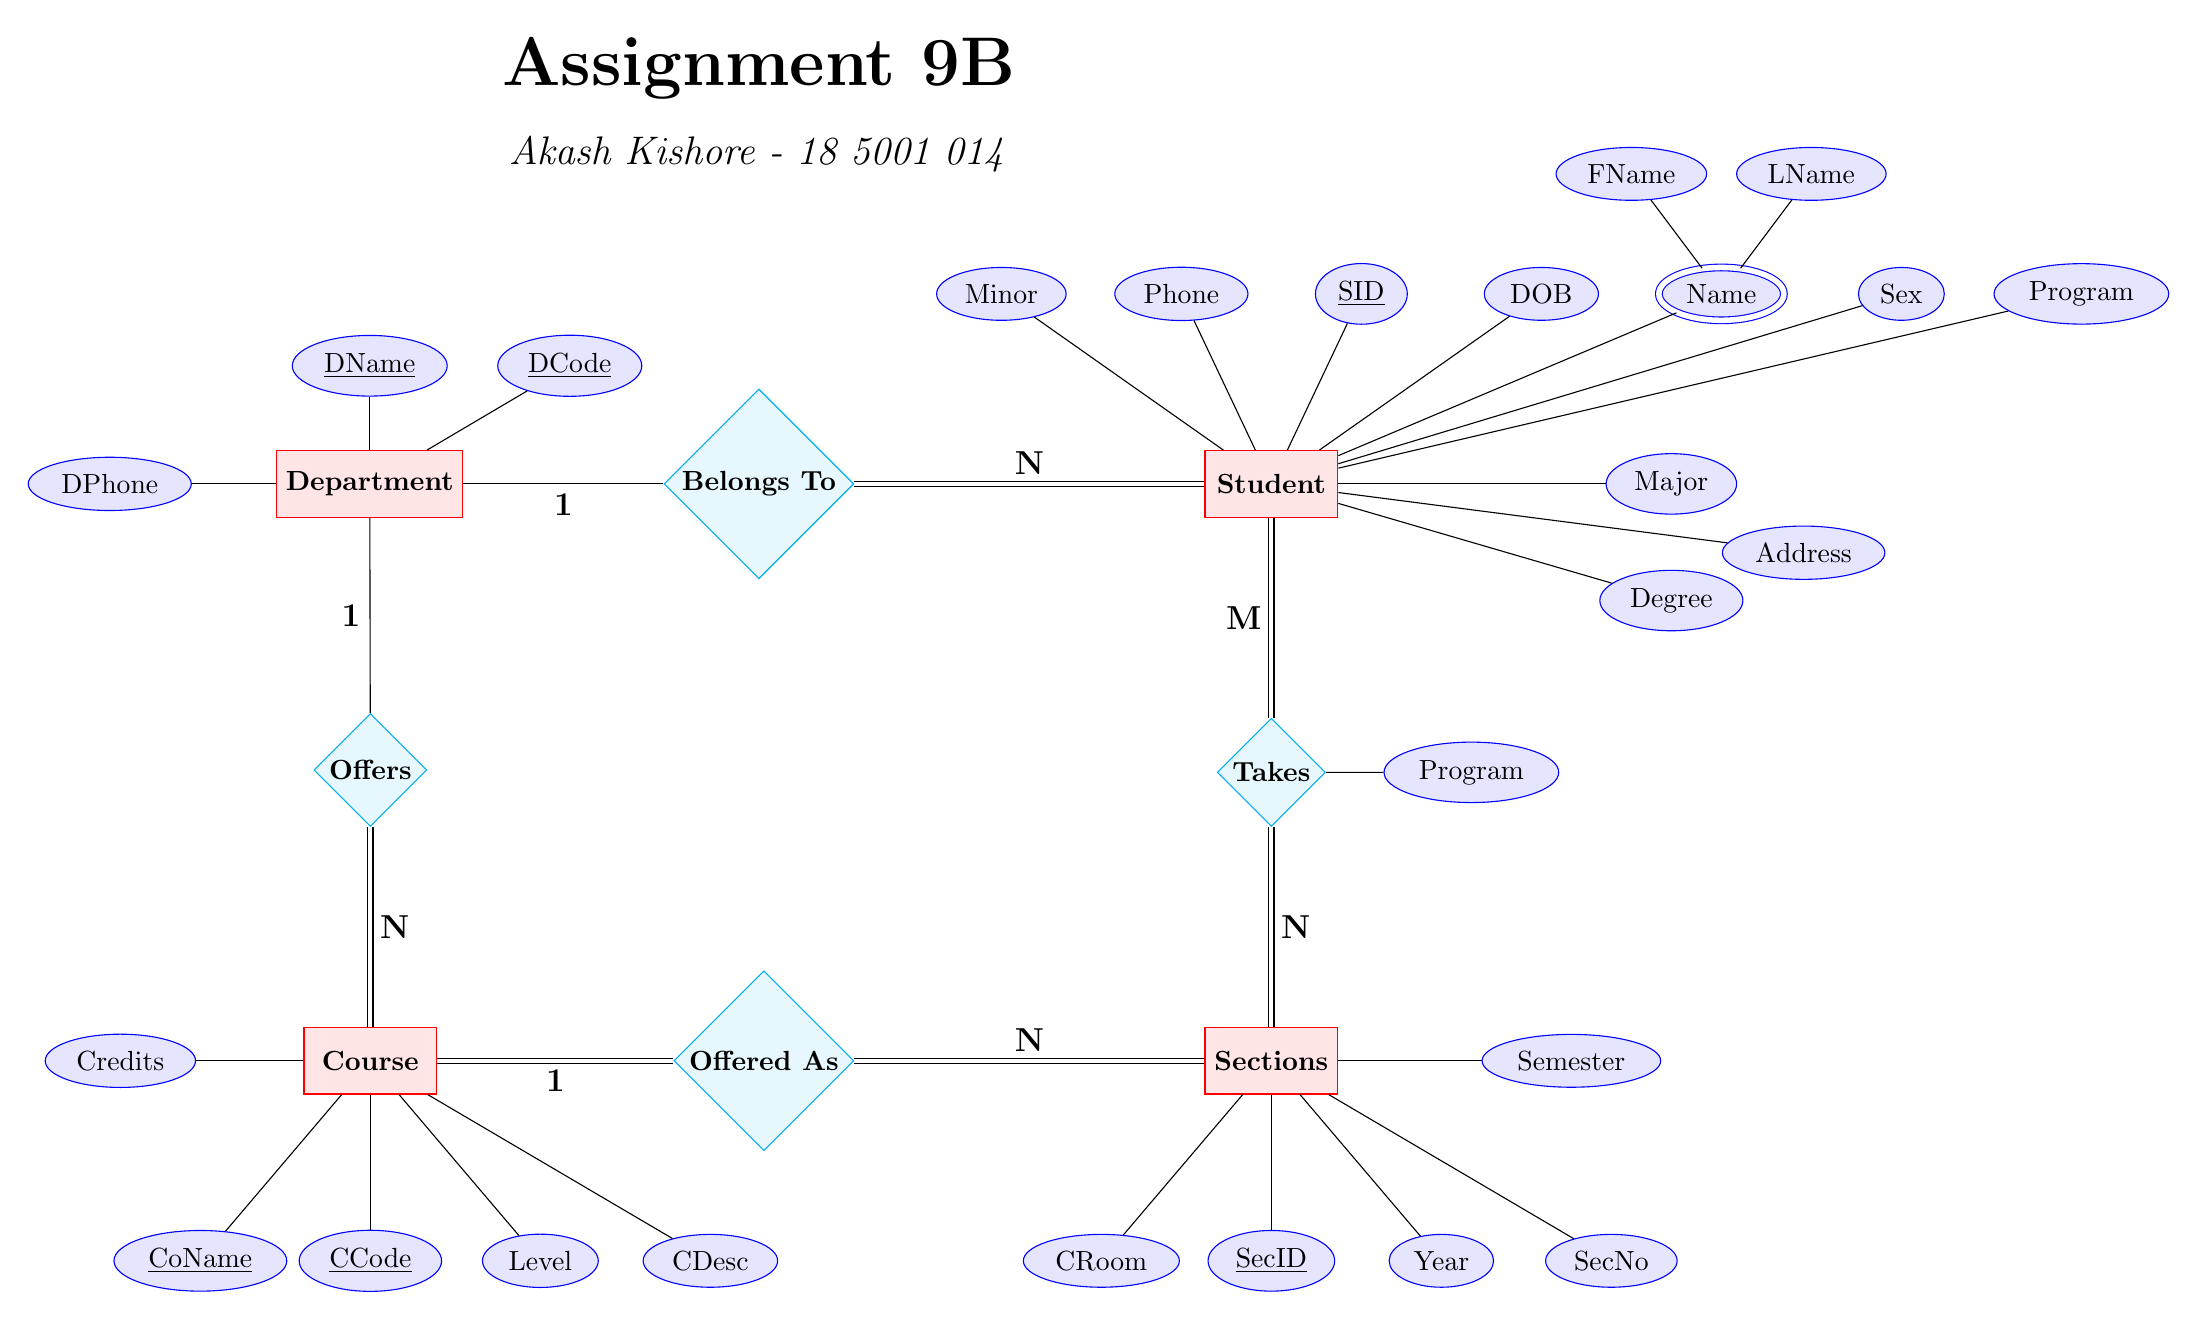
\begin{tikzpicture}[auto,node distance=1in]
%\tikzstyle{every pin edge}=[draw]
\node[entity] (department)  {\textbf{Department}} [grow=up,sibling distance=1in]
child {node[attribute] {\underline{DCode}}}
child {node[attribute] {\underline{DName}}}
child[grow=left,level distance=1.3in] {node[attribute] {DPhone}};
%child[grow=right,sibling distance=7cm] {node[attribute] {color}}

\node[relationship] (belongs) [right=1in of department] {\textbf{Belongs To}};

\node[entity] (student) [right=1.75in of belongs] {\textbf{Student}} [grow=up,level distance=0.95in,sibling distance=0.9in]
child {node[attribute] {Program}}
child {node[attribute] {Sex}}
child {node[multi attribute] {Name} child[level distance=0.6in] {node[attribute] {LName}} child[level distance=0.6in] {node[attribute] {FName}}}
child {node[attribute] {DOB}}
child {node[attribute] {\underline{SID}}}
child {node[attribute] {Phone}}
child {node[attribute] {Minor}}
child[grow=right,level distance=2in] {node[attribute] (major) {Major}}
child {node[attribute] (degree) [below=0.7cm of major]{Degree}}
child {node[attribute] [below right=0.5cm of major] {Address}}
%child[grow=right,level distance=1.2in] 
;


\node[relationship] (takes) [below=1in of student] {\textbf{Takes}}[grow=right,level distance=1in]
child {node[attribute] {Program}};


\node[entity] (section) [below=1in of takes] {\textbf{Sections}} [grow=down,level distance=1in,sibling distance=0.85in]
child[grow=right,level distance=1.5in] {node[attribute] {Semester}}
child {node[attribute] {CRoom}}
child {node[attribute] {\underline{SecID}}}
child {node[attribute] {Year}}
child {node[attribute] {SecNo}}
;


\node[relationship] (offeredas) [left=1.75in of section] {\textbf{Offered As}};


\node[entity] (course) [left=1.18in of offeredas] {\textbf{Course}} [grow=down,level distance=1in,sibling distance=0.85in]
child[grow=left,level distance=1.25in] {node[attribute] {Credits}}
child {node[attribute] {\underline{CoName}}}
child {node[attribute] {\underline{CCode}}}
child {node[attribute] {Level}}
child {node[attribute] {CDesc}}
;

\node[relationship] (offers) [above=1in of course] {\textbf{Offers}};


\node[entity,draw=white,fill=white] (title) [above=1.4in of belongs] {\Huge \textbf{Assignment 9B }};

\node[entity,draw=white,fill=white] (title) [above=1in of belongs] {\Large \textit{Akash Kishore - 18 5001 014}};


%Participations and Cardinality Ratios

\path (belongs) edge node {\large \textbf{1}} (department) edge[total] node {\large \textbf{N}} (student);

\path (offers) edge node {\large \textbf{1}} (department) edge[total] node {\large \textbf{N}} (course);

\path (offeredas) edge[total] node {\large \textbf{1}} (course) edge[total] node {\large \textbf{N}} (section);

\path (takes) edge[total] node {\large \textbf{M}} (student) edge[total] node {\large \textbf{N}} (section);



\end{tikzpicture}
\end{document}